\documentclass[xcolor=svgnames]{beamer}
\mode<presentation>
{
      \setbeamertemplate{footline}[page number]
      \setbeamercovered{transparent}
      \setbeamertemplate{navigation symbols}{}
      \usecolortheme[named=DarkGreen]{structure}
}

\usepackage[english]{babel}
\usepackage{times}
\usepackage{url}
\usepackage{CJKutf8}
\usepackage{graphics}
\usepackage{amsmath}
\usepackage{listings}
\lstset{breakatwhitespace,
language=C,
columns=fullflexible,
keepspaces,
breaklines,
tabsize=3,
showstringspaces=false,
extendedchars=true}


\AtBeginSubsection[]
{
    \begin{frame}<beamer>{Outline}
    \tableofcontents[currentsection,currentsubsection]
    \end{frame}
}


\begin{document}
\begin{CJK*}{UTF8}{gbsn}


\title{OS概念与Linux内核代码分析之三:进程同步}
\author{李中国}
\institute{苏州大学计算机科学与技术学院} 

\begin{frame}
\maketitle
\end{frame}

\begin{frame}{内容提要}
\tableofcontents[pausesections]
\end{frame}

\section{原子操作}

\begin{frame}[fragile]%{Linux内核关键数据结构:list}
\frametitle{什么是原子操作?}
\begin{block}{原子操作的定义}
整个操作(计算机执行的指令序列)不可分割,要么全部做完,要么全部不做。
\end{block}
\begin{block}{不能保证是原子操作的例子}
\begin{verbatim}
a = a + 1;
a++;
\end{verbatim}
这些C语言语句都涉及read-modify-write这样的机器指令序列,因而不是原子操作。
\end{block}
\begin{block}{原子操作的例子}
\begin{itemize}
\item 如果某指令不涉及内存地址,则肯定是原子操作
\item Intel平台上,如果指令前面有lock标记(0xf0), 则是原子操作
\end{itemize}
\end{block}
\end{frame}

\defverbatim[colored]\lstatomict{
\begin{lstlisting}[tabsize=8,basicstyle=\ttfamily]
typedef struct __atomic_t { 
    volatile int counter; 
} atomic_t;

#define ATOMIC_INIT(i)  { (i) }

#define atomic_read(v)  ((v)->counter)

static __inline__ void atomic_add(int i, atomic_t *v)
{
    __asm__ __volatile__(
        LOCK "addl %1,%0"
        :"=m" (v->counter)
        :"ir" (i), "m" (v->counter));
}
\end{lstlisting}

}
\begin{frame}[fragile]%{Linux内核关键数据结构:list}
\frametitle{Linux内核中的atomic\_t类型及操作}
\begin{block}{include/asm-x86\_64/atomic.h }
\lstatomict
\end{block}
\end{frame}

\section{实现分段的硬件装置}

%\subsection{段选择符及段寄存器}

\begin{frame}[fragile]
\frametitle{内存寻址: 实模式与保护模式}
\begin{description}
\item[实模式] 寻址采用和8086相同的16位段和偏移量,最大寻址空间1MB(4*seg + off),最大分段64KB。
\item[保护模式] 寻址采用32位段和偏移量,最大寻址空间4GB,最大分段4GB (Pentium Pre及以后为64GB)。
\end{description}
\begin{block}{两种模式的主要区别}
二者的根本区别是进程内存受保护与否。实模式下系统程序和用户程序没有区别对待,每一个指针都是指向"实在"的物理地址。
\end{block}
\end{frame}

\begin{frame}[fragile]
\frametitle{段选择符及段寄存器}
\begin{block}{段选择符}
逻辑地址由16位的段号(segment ID)和32位段内偏移(offset)组成.
其中段号在Intel平台上称为段选择符(segment selector).
其16个二进制位中存放信息如下图。


\includegraphics[width=0.7\textwidth]{selector.png}
\end{block}
\begin{block}{段寄存器}
CPU内部专门用来存放段选择符的存储单元。共有六个:cs, ss, ds, es, fs, gs. 其中: 
\begin{description}
\item[cs] 代码段寄存器(程序指令)
\item[ss] 栈段寄存器(运行时的栈)
\item[ds] 数据段寄存器(全局及静态变量)
\end{description}
\end{block}
\end{frame}


\begin{frame}[fragile]
\frametitle{段描述符}
内存分段后,每个段表项存放相应段的性质(如地址、存放内容的类型等).
段表项在Intel平台上称为段描述符(segment descriptor).
有两类段表: 全局段表(GDT,系统中仅有一个), 局部段表(LDT,每个进程可以单独有一个).
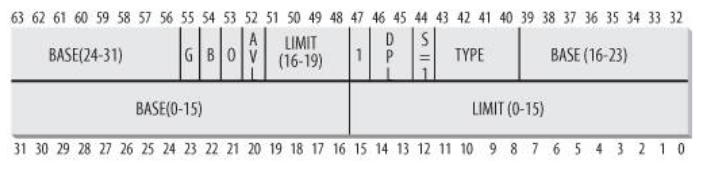
\includegraphics[width=0.7\textwidth]{descriptor.png}
\begin{block}{几个关键字段}
\begin{description}
\item[Base] 该段起始地址
\item[Limit] 该段总长度
\item[G] 标记Limit字段的单位是1字节还是4096字节
\item[Type] 该段类型(代码、数据、其它)
\end{description}
\end{block}
\end{frame}


\begin{frame}[fragile]
\frametitle{段选择符的三个字段}
%\begin{block}{}
%\end{block}
%\begin{block}{思考}
%\end{block}
\begin{description}
\item[index] 用于对段表进行索引
\item[TI] 用于指定该选择符对应GDT(TI=0)还是LDT(TI=1)
\item[RPL] 记录CPU权限状态(核心态/用户态)
\end{description}


\includegraphics[width=0.7\textwidth]{selector.png}
\end{frame}

\begin{frame}[fragile]
\frametitle{从逻辑地址到线性地址的映射}
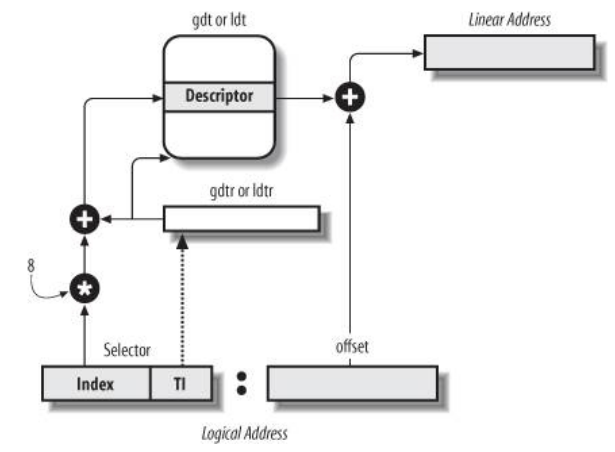
\includegraphics[width=0.8\textwidth]{segunit.png}
\end{frame}

\section{Linux + Intel平台上的内存分页}

\begin{frame}[fragile]
\frametitle{Intel平台上的分页技术}
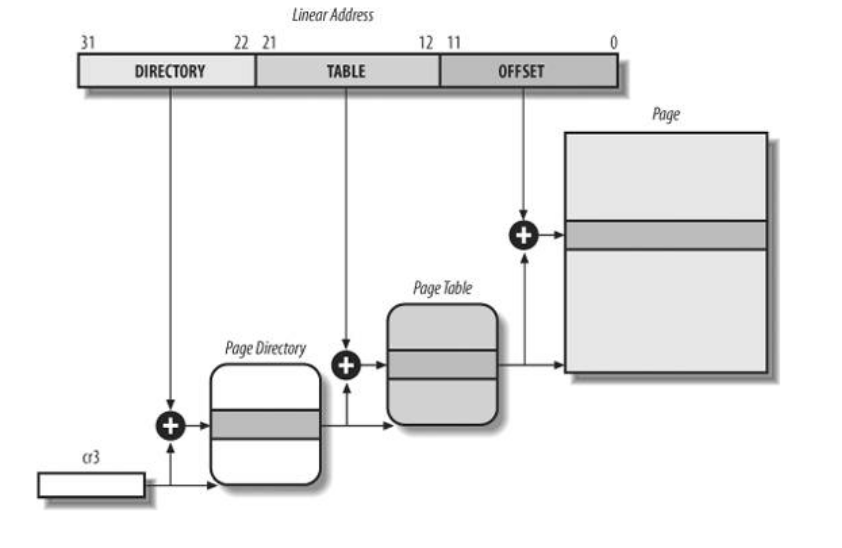
\includegraphics[width=0.8\textwidth]{regpaging.png}

cr3寄存器用于存放当前进程的page directory(第一级页表).
\end{frame}

\begin{frame}[fragile]
\frametitle{Intel平台上的扩展分页模式}
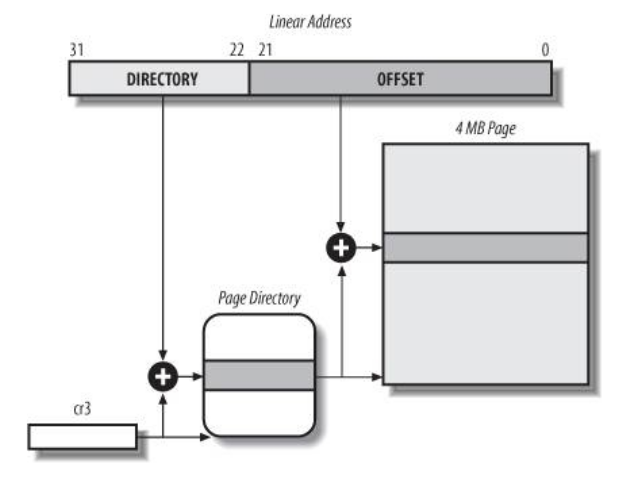
\includegraphics[width=0.8\textwidth]{extpaging.png}

扩展分页模式下,页面大小为4M,用于处理大块连续地址空间,
以节省页表所占空间及TLB空间。
\end{frame}

\begin{frame}[fragile]
\frametitle{分页的实际例子}
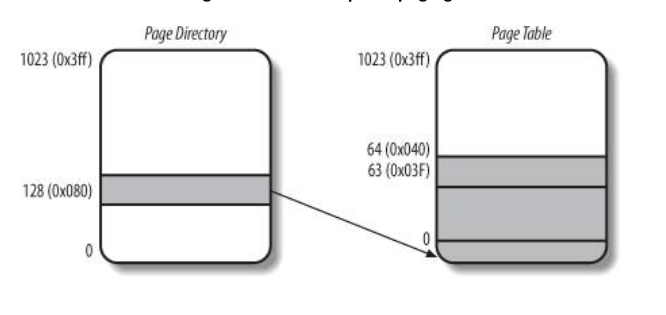
\includegraphics[width=0.8\textwidth]{examplepaging.png}

假设内核把从\verb|0x20000000|到\verb|0x2003ffff|之间的线性地址(共64页)分配给某进程。
\begin{itemize}
\item 该段地址最高10位均为\verb|0010000000|, 即\verb|0x080|(十进制128),因此第一级页表只有一个页表项有效。
\item 该段地址中间10位范围为0 -- \verb|0x03f|(即0 -- 63). 所以第二级页表中开头64个页表项有效。(图示灰色区域)
\item 给定线性地址\verb|0x20021406|,如何确定其对应的物理地址?
\end{itemize}

\end{frame}

\begin{frame}[fragile]
\frametitle{Linux的分页技术实现方式}
为了能够同时处理32位和64位机器的分页方式, Linux创造性地使用4级分页来同时适应硬件1--4级分页需求。

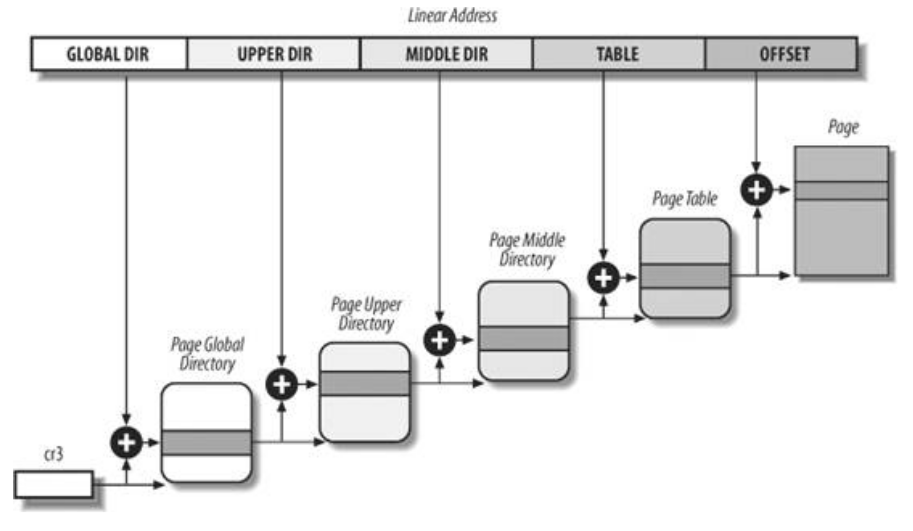
\includegraphics[width=0.8\textwidth]{linuxpaging.png}
\end{frame}

\begin{frame}[fragile]
\frametitle{Linux的分页技术实现方式}
上图中共有四种类型的页表:
\begin{description}
\item[Page Global Directory]
\item[Page Upper Directory]
\item[Page Middle Directory]
\item[Page Table]
\end{description}
对于32位机器,2级页表就够了,此时,Linux把Page Upper Directory和Page Middle Directory两字段对应的地址长度设置为0.

\end{frame}

\begin{frame}[fragile]
\frametitle{有关线性地址各个字段及页表项的一些宏}
\begin{block}{include/asm-x86\_64/\{page.h, pgtable.h\}}
\begin{itemize}
\item \verb|PAGE_SHIFT|, \verb|PAGE_SIZE|, \verb|PAGE_MASK|
\item \verb|PMD_SHIFT|, \verb|PMD_SIZE|, \verb|PMD_MASK|
\item \verb|PUD_SHIFT|, \verb|PUD_SIZE|, \verb|PUD_MASK|
\item \verb|PGDIR_SHIFT|, \verb|PGDIR_SIZE|, \verb|PGDIR_MASK|
\end{itemize}
如何根据\verb|SHIFT|, \verb|SIZE|, \verb|MASK|的关系定义上述宏?
\end{block}
\begin{block}{include/asm-x86\_64/pgtable.h}
\begin{itemize}
\item \verb|PTRS_PER_PTE|
\item \verb|PTRS_PER_PMD|
\item \verb|PTRS_PER_PUD|
\item \verb|PTRS_PER_PGD|
\end{itemize}
需要注意32位和64位机器(页表级数不同)上述值的差别。
\end{block}
\end{frame}


\defverbatim[colored]\lstptet{
\begin{lstlisting}[tabsize=8,basicstyle=\ttfamily]
typedef struct { unsigned long pte; } pte_t;
typedef struct { unsigned long pmd; } pmd_t;
typedef struct { unsigned long pud; } pud_t;
typedef struct { unsigned long pgd; } pgd_t;
\end{lstlisting}
}
\begin{frame}[fragile]
\frametitle{处理页表的函数}
\begin{block}{各类页表项的定义: include/asm-x86\_64/page.h}
\lstptet

注: Linux内核以后缀\verb|_t|表示系统自定义类型。
\end{block}
\begin{block}{思考}
为什么不直接用\verb|unsigned long|表示各类页表项?
\end{block}
\end{frame}

\defverbatim[colored]\lstconversions{
\begin{lstlisting}[tabsize=8,basicstyle=\ttfamily]
#define pte_val(x)  ((x).pte)
#define pmd_val(x)  ((x).pmd)
#define pud_val(x)  ((x).pud)
#define pgd_val(x)  ((x).pgd)
#define pgprot_val(x)   ((x).pgprot)

#define __pte(x) ((pte_t) { (x) } )
#define __pmd(x) ((pmd_t) { (x) } )
#define __pud(x) ((pud_t) { (x) } )
#define __pgd(x) ((pgd_t) { (x) } )
#define __pgprot(x) ((pgprot_t) { (x) } )
\end{lstlisting}
}
\begin{frame}[fragile]
\frametitle{处理页表的函数}
\begin{block}{include/asm-x86\_64/page.h}
\lstconversions
\end{block}
\end{frame}

%\begin{frame}[fragile]
%\frametitle{针对list结构的操作举例: list\_add}
%%\lstadd
%\end{frame}
%
%\begin{frame}[fragile]
%\frametitle{创建进程: do\_fork函数的实现}
%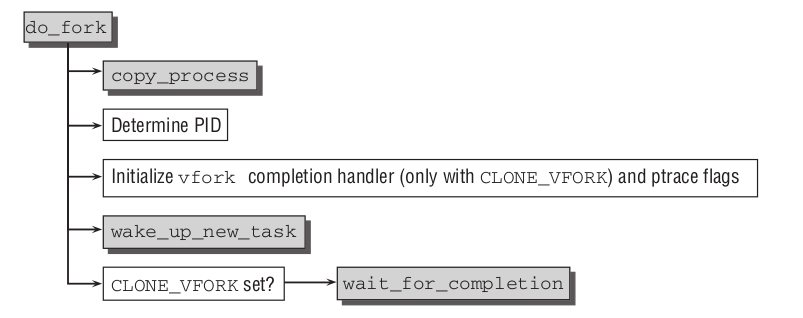
\includegraphics[width=1.0\textwidth]{dofork.png}
%\end{frame}

\end{CJK*}
\end{document}
